%%%%%%%%%%%%%%%%%%%%%%%%%%%%%%%%%%%%%%%%%%%%%%%%%%%%%%%%%%%%%%%%
\begin{comment}

* Maintain 80 characters / line.
 
* too much ``''s make the sentence look scattered and visually less recognizable. ``e.g.'' also.

* \em, \bf, \it are all obsolete \TeX primitives, and it does not take effect properly --- for example, {\bf {\it aaa}} shows ``aaa'' in italic but NOT IN BOLD. Use \emph{}, \textit{}, \textbf{} and so on.

* always use \ff, \fd, \cea, \pr, \mv , and do not use it directly, e.g. FF, FD/LAMA2011, etc. 

* use of footnotes should be minimized.

* IPC2011 should always be \ipc . The definition can later be modified in abbrev.sty .

* prefer separated words over hyphened words. domain
  independent>domain-independent, planner independent >
  planner-independent.

* Table, Figure, Fig., should not be used directly. Always use \refig and \reftbl. When the development flag is enabled, direct use of \ref signals an error.

* Caption ends with a period.
\end{comment}

%%%%%%%%%%%%%%%%%%%%%%%%%%%%%%%%%%%%%%%%%%%%%%%%%%%%%%%%%%%%%%%%

\begin{abstract}
% intentionally made different from the 1st-order symbol paper, writing style is also different
While domain-independent classical planning is an active area of research,
its applicability to the real-world tasks are limited to those precisely modeled by human.
Recently, \latentplanner \cite{Asai2018} combined classical planning with deep-learning
to obtain the symbolic description of the image based domain.
In this paper, we address a problem in their preliminary implementation of \latentplanner,
specifically the uninformative / random propositions in the latent / symbolic encoding,
and provides a remedy for it.
%
Those uninformative propositions become true or false depending on the coin flip,
which means that
% some of the propositiosn in the latent layer may not carry significant meaning / affect the output.
% While this is not problematic for encoding/decoding, from search/planning perspective this is a major problem,
% because this means that 
 a single state can have multiple propositional representations and no longer the
unique representation amenable for search algorithms.
% 
One effective way to suppress this behavior is to have an additional regularization
for the latent propositions which guides the training so that 
% toward sparser, disentangled propositional representation,
unused propositions tends to be 0.
 % 
We empirically show that this ``Zero-Suppressed SAE''
has lower variance encoding (more stable propositions) for each single state
and improves the success rate of \latentplanner.
% XXX TODO: unknown if it is possible
[TODO]
Furthermore, we show that this Zero-Suppressed SAE can act like a declarative knowledge base
where you incrementally assign new knowledge to unused propositions.
We show this by retraining an existing network
with a mixture of the existing and new dataset, and demonstraining that
it can encode both environments.
\end{abstract}

\section{Introduction}

Recently, Latplan system \cite{Asai2018} successfully
connected a subsymbolic neural network system and a symbolic Classical Planning system
to solve various visually presented puzzle domains.
% In contrast to the work by Konidaris et. al. (\citeyear{KonidarisKL14}),
% Latplan is a straightforward NN built upon a \lsota framework.
The system generates a set of propositional variables \emph{from nowhere},
i.e., by unsupervised learning without manual tagging and only from the image inputs.
% 
The system provides a bidirectional mapping between images and propositional states,
solves the propositional problem using a classical planner Fast Downward \cite{Helmert04},
then returns a sequence of images that solves the puzzle,
by decoding the intermediate propositional states back to images.
 
However,
neural networks in general do not have a strong guarantee on the learned results,
and thus the propositional representations learned by Latplan have several problems.
% We noticed from the public code of Latplan available on Github that
First, the propositional symbols generated by Latplan is not always
``stable'', i.e., some propositions may not remain true or false given the same image input
and rather flip randomly.
This means that a single image maps to multiple propositonal states and the mapping is
no longer 1-to-1.
% 
At the same time, these unstable propositions do not affect the output, therefore they are
``unused'' and ``uninformative'', i.e.,
whether the proposition is true or false does not affect the output image decoded from the propositional state.
In fact, in the appendix section in the Arxiv version of the original paper,
the authors state that they use the \emph{state augmentation} technique
which circumvent this problem by sampling states from the same image multiple times.

Second, the system is sensitive to the hyperparameter, and if inappropriate parameter
is used, planning fails without solution or returns a suboptimal or even wrong solution.
Specifically, if we set the number of propositions ($=$ number of nodes in the latent layer) too high, the network
has an excessive capacity which results in too many unused propositions,
which makes the state space graph disconnected.
This happens because some edge is connected to only one variant of
the possible propositional representations of the image.

\begin{figure}[htb]
 \centering
 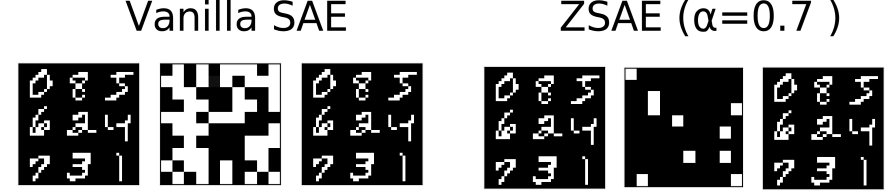
\includegraphics{img/zsae-overview.pdf}
 \caption{
Conceptual images of Vanilla SAE and Zero-Suppressed SAE (ZSAE) encoding a MNIST 8-puzzle state, with 100 propositions.
ZSAE obtains a representation that has fewer true bits.}
 \label{zsae-overview}
\end{figure}

To address these problems,
we introduce an additional regularization penalty function for the neural network 
that makes the learned propositions more ``stable''. In the resulting neural network,
Zero-Suppressed State AutoEncoder (ZSAE, \refig{zsae-overview}), this penalty function
guides the network optimization so that unused propositions tend to 
take the value of zero (false) instead of random values,
resulting in a more stable representation.
The stability can be measured by taking the variance of the representation from the same set of inputs.
We also show that a more stable representation results in a higher success rate of classical planning.

Also, with this additional penalty, the number of bits required to represent the same function
is minimized and the network becomes less sensitive to the hyperparameters.

The idea behind ZSAE is similar to the Zero-Suppressed Binary Decision Diagram \cite{minato1993zero},
which is a variant of Binary Decision Diagram \cite{bryant1986graph} with an alternative node reduction rule:
Nodes whose 1-edge going to constant 0-node is pruned.
With a similar intent, we show that we can similarly prune some unused neurons
that has a constant activation of zero
that were resulted from our additional regularization penalty.
This reduces the memory usage as well as the inference time of the neural network.

The rest of the paper is organized as follows.
In \refsec{background}, we introduce Laplan \cite{Asai2018} and its State AutoEncoder (SAE).
Next, we describe the problematic behavior of this vanilla SAE in more details (\refsec{issues}).
Next we introduce Zero-Suppressed SAE (ZSAE), the main contribution of this paper (\refsec{zsae}).
We empirically evaluate the stability of the propositions generated by Vanilla SAE and ZSAE,
as well as showing results indicating various other advantages of ZSAE (\refsec{evaluation}).
We finally conclude the paper with related work and future remark (\refsec{conclusion}).


\section{Preliminaries}
\label{background}

\textbf{Symbol Grounding} is an unsupervised process of establishing a mapping
from huge, noisy, continuous, unstructured inputs
to a set of compact, % clean
discrete, identifiable (structured) entities, i.e., symbols \cite{Asai2018}.
For example, PDDL has six kinds of symbols: Objects, predicates, propositions, actions, problems and domains (\reftbl{tab:type-of-symbols}).
Each type of symbol requires its own mechanism for grounding.
For example, the large body of work in the image processing community on recognizing 
objects (e.g. faces) and their attributes (male, female) in images, or scenes in videos (e.g. cooking)
can be viewed as corresponding to grounding the object, predicate and action symbols, respectively.

\begin{table}[tbp] 
\centering
\relsize{-1}
\begin{tabular}{ll}
Types of symbols & \\
\hline
Object symbols    & \textbf{panel7, x\(_{\text{0}}\), y\(_{\text{0}}\)} \ldots{}               \\
Predicate symbols & (\textbf{empty} ?x ?y) (\textbf{up} ?y\(_{\text{0}}\) ?y\(_{\text{1}}\))   \\
Propositions      & \textbf{empty\(_{\text{5}}\)} = (empty x\(_{\text{2}}\) y\(_{\text{1}}\)) (6th application) \\
Action symbols    & (\textbf{slide-up} panel\(_{\text{7}}\) x\(_{\text{0}}\) y\(_{\text{1}}\)) \\
Problem symbols   & \textbf{eight-puzzle-instance1504}, etc.                                   \\
Domain  symbols   & \textbf{eight-puzzle}, \textbf{hanoi}                                      \\
\hline
\end{tabular}
\caption{6 types of symbols in a PDDL definition.}
\label{tab:type-of-symbols}
\end{table}

\textbf{\latentplanner} \cite{Asai2018} is a framework for
\emph{domain-independent image-based classical planning}.
\latentplanner addresses two of the 6 types of symbols listed in \reftbl{tab:type-of-symbols},
namely propositional and action symbols.

Classical planners such as FF \cite{hoffmann01} or
FastDownward \cite{Helmert04} takes a PDDL model as an input, which
specifies the state representation, the initial state, the goal
condition and the transition rules in the form of first order logic
formula.  In contrast, \latentplanner learns the state representation as well as the transition rules
entirely from the image-based observation of the environment with deep neural networks.
% , and also claims to extend its capability on text/audio-based dialog data in the future.
The system was shown to solve various puzzle domains, such as 8-puzzles or Tower of Hanoi,
which are presented in a form of noisy, continuous visual depiction of the environment.

\begin{figure}[htb]
 \centering
 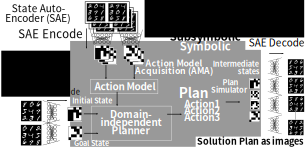
\includegraphics[width=\linewidth]{img/planning.pdf}
 \caption{Classical planning in latent space:
It uses the learned State Autoencoder (\refig{sae}) to convert pairs of images $(\before,\after)$ to symbolic transitions, from which the AMA component generates an action model.
It also encodes the initial and goal state images into symbolic initial/goal states.
A classical planner finds the symbolic solution plan.
Finally, intermediate states in the plan are decoded back to a human-comprehensible image sequence.}
\label{fig:overview}
\end{figure}

\latentplanner takes two inputs.
The first input is the \emph{transition input} $Tr$, a set of pairs of raw data.
Each pair $tr_i=(\before_i, \after_i) \in Tr$ represents a transition of the environment before and after some action is executed.
The second input is the \emph{planning input} $(i, g)$, a pair of raw data, which corresponds to the initial and the goal state of the environment.
The output of \latentplanner is a data sequence representing the plan execution that reaches $g$ from $i$.
While the original paper uses an image-based implementation (``data'' = raw images),
the type of data is arbitrary as long as it is compatible to neural network.

% Emphasize the type of symbol, as readers are not familier with or haven't deeply thought about symbols
% \subsection{SAE for Propositional Symbol Grounding}

\latentplanner works in 3 phases.
In Phase 1, a \emph{State Autoencoder} (SAE) (\refig{sae}) learns a bidirectional mapping between raw data (e.g., images)
 and propositional states from a set of unlabeled, random snapshots of the environment.
The $Encode$ function maps images to propositional states, and $Decode$ function maps the propositional states back to images.
After training the SAE from $\braces{\before_i, \after_i\ldots}$,
it applies $Encode$ to each $tr_i \in Tr$ and obtain $(Encode(\before_i),$ $Encode(\after_i))=$ $(s_i,t_i)=$ $\overline{tr}_i\in \overline{Tr}$,
the symbolic representations (latent space vectors) of the transitions.

In Phase 2, an AMA method learns an action model from $\overline{Tr}$ in an unsupervised manner.
The original paper propose two approaches: AMA$_1$ is an oracular model which directly generates a PDDL without learning,
and AMA$_2$ is a neural machine learning model that can learn from examples.

In Phase 3, a planning problem instance is generated from the planning input $(i,g)$.
These are converted to symbolic states by the SAE, and the symbolic planner solves the problem.
For example, an 8-puzzle problem instance consists of an image of the start (scrambled) configuration of the puzzle ($i$), and an image of the solved state ($g$).

Since the intermediate states comprising the plan are SAE-generated latent bit vectors, the ``meaning'' of each state (and thus the plan) is not clear to a human observer.
However, in the final step, \latentplanner obtain a step-by-step visualization of the plan execution
by $Decode$'ing the latent bit vectors for each intermediate state.
This necessitates the bidirectionality of the mapping between the input and the propositional states.

\begin{figure}[htb]
 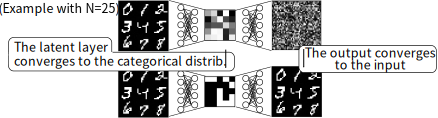
\includegraphics[width=\linewidth]{img/train-state-ae.pdf}
 \caption{State AutoEncoder, a
 Variational AutoEncoder \cite{kingma2014semi} using Gumbel-Softmax \cite{jang2016categorical} reparametrization in its
 latent layer.}
 \label{sae}
\end{figure}

\subsection{SAE as a Variational AutoEncoder using Gumbel-Softmax}

The key concept of the SAE in \latentplanner is the use of Gumbel-Softmax \cite{jang2016categorical}
reparameterization trick in the latent activation of Variational AutoEncoder.
This allows SAE to obtain the
discretized binary representation, and \latentplanner uses this
discrete vector as the state representation for classical planning.

An Autoencoder (AE) is a type of feed-forward neural network that learns an identity function whose output matches the input \cite{hinton2006reducing}.
% It is a form of unsupervised learning as it does not require the labels.
Its intermediate layer (typically smaller than the input) has a compressed, \emph{latent representation} of the input.
% AEs are commonly used for pretraining a NN.
AEs are trained by backpropagation (BP) to minimize the reconstruction loss, the distance between the input and the output according to a distance function such as Euclidean distance.
NNs, including AEs, typically have continuous activations and integrating them with propositional reasoners is not straightforward.

A Variational Autoencoder (VAE) \cite{kingma2013auto} is a type of AE that forces the \emph{latent layer} (the most compressed layer in the AE) to follow a certain distribution (e.g., Gaussian).
% While initially proposed for enforcing Gaussian distributions, VAEs have been used to enforce arbitrary types of distribution (notably by Generative Adversarial Network \cite{goodfellow2014generative,makhzani2015adversarial}). 
Since the random distribution is not differentiable (BP is not applicable), VAEs use \emph{reparametrization tricks}, which decompose the target distribution into a differentiable and a purely random distribution (the latter does not require the gradient).
For example, the Gaussian $N(\sigma,\mu)$ is decomposed to $\mu+\sigma N(1,0)$, where $\mu,\sigma$ are learned.
In addition to the reconstruction loss, VAE should also minimize the variational loss (the difference between the learned and the target distributions) measured by, e.g.,  KL divergence.

Gumbel-Softmax (GS) is a re\-para\-metri\-zation trick \cite{jang2016categorical} for categorical distribution.
It continuously approximates Gumbel-Max \cite{maddison2014sampling}, a method for drawing categorical samples.
Assume the output $z$ is a one-hot vector, e.g. if the domain is $D=\braces{a,b,c}$, $\brackets{0,1,0}$ represents ``b''.
The input is a class probability vector $\pi$, e.g. $\brackets{.1,.1,.8}$.
Gumbel-Max draws samples from $D$ following $\pi$:
% \[
 $z_i \equiv [ i = \arg \max_j (g_j+\log \pi_j)\ ?\ 1 : 0 ]$
% \]
where $g_j$ are i.i.d samples drawn from Gumbel$(0,1)$ \cite{gumbel1954statistical}.
Gumbel distribution is a random distribution that can be sampled from $-\log (-\log (\text{Uniform}(0,1)))$, where
$\text{Uniform}(0,1)$ is a uniform random distribution between 0 and 1.
Gumbel-Softmax approximates argmax with softmax to make it differentiable:
% \[
$z_i = \text{Softmax}((g_i+\log \pi_i)/\tau)$.
% \]
``Temperature'' $\tau$ controls the magnitude of approximation, which is annealed to 0 by a certain schedule.
The output of GS converges to a discrete one-hot vector when $\tau\approx 0$.

In a vanilla SAE \cite{Asai2018}, there are $N$ units of Gumbel-Softmax
for 2 categories in the latent layer, resulting in a $N\times 2$ matrix,
where $N$ specifies the number of propositional variables in the latent
state representation. The latent layer can be written as
$z_{ij}$ where $j\in \braces{0,1}$ and $1\leq i \leq N$.  When the
temperature $\tau$ is low, one of $z_{i0}$ or $z_{i1}$ takes the value
of 1 and another one takes the value of 0 (one-hot vector).  A binary
propositional vector can thus be extracted by taking the first row,
$\parens{z_{00}\ldots z_{N0}}$.

\subsection{Regularization in Neural Network}

\emph{Regularization} is an imporatnt concept in machine learning
that limits the representation capacity of the nueral network by adding a constraint
to the optimization criteria of the neural network that is minimzied by algorithms like Stochastic Gradient Descent.
Regularization trades the (training) performance with generalization capability (testing performance, robustness to
unseen data points) in order to suppress the overfiting.

Notable regularization techniques used for neural networks include
$l_1$ or $l_2$ regularization that penalizes the sum / square sum of the
activations, or Dropout \cite{srivastava2014dropout}, that randomly drops some neurons so
that each pattern is more strongly associated with a fewer set of nodes.

% It is necessary for the mapping to be bidirectional, because the
% propositional variables are machine-generated symbols, and also the
% resulting plan (returned as a sequence of propositional states) should
% be decoded back to real-world images which are interpretable for humans.

% \latentplanner also learns the action model using a neural action model acquisition method AMA$_2$,
% but we omit the details due to space limitation.

\section{Issues in the State Representation in the Vanilla SAE}
\label{issues}

The issues in a vanilla SAE is that the class probability could be
neutral for class ``true'' and class ``false'', and the resulting value
of a proposition is random (\refig{unstable}).
The randomness of the vanilla SAE comes from
the Gumbel distribution $-\log (-\log (\text{Uniform}(0,1)))$ which includes
a uniform random distribution.
This causes several problems from the symbolic reasoning (classical planning) point of view.

\begin{figure}[htb]
 \centering
 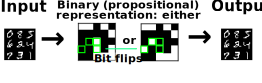
\includegraphics{img/unstable.pdf}
 \caption{Propositions found by Vanilla SAE may contain several uninformative bits
 that flip randomly and do not affect the output.}
 \label{unstable}
\end{figure}

First, the algorithms that run on the state space generated based on these propositional vectors
are confused by many variation of the essentially identical real world states.
It could visit variations of the same real world state that are encoded into different propositional vector,
however the duplicate detection could not detect it since it completely relies on the atomiticy and deteminisim of the
proposition. This slows down the search by increasing the number of nodes that can be reachable from the initial state
while these are essentially unnecessary amount of work.

\begin{figure}[htb]
 \centering
 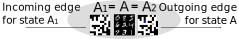
\includegraphics{img/disconnected.pdf}
 \caption{Two random variations of propositional encoding for a single real-world state could make the state space graph disconnected.}
 \label{disconnected}
\end{figure}

Secondly, the state space could be disconnected due to such random variations (\refig{disconnected}).
Certain state transition (edge) may be only reached via a single variation of the real world state, and is not connected to the
other variation of the propositional state that represents the same real-world state.

We note that while some values in the latent layer are random, most of values are not.
These unused, uninfoirmative bits are generated because hte network has toom uch capacity to 
model the entire state space, i.e. they appear when we specify the number of proposition $N$ too large.
If we reduces $N$ while maintaining the reconstruction capability of the SAE, the number of uninformative bits
reduces.
On the contrary, if we specify $N$ too small, it lacks the capacity to represent the state space
and the SAE is no longer able to reconstruct the
real world image.
As a result, we face a hyperparameter tuning problem: Too large $N$ causes a disconnected state space graph,
and too small $N$ does not converge on the dataset.

To tackle this problem, we propose Zero-Suppressed State Autoencoder (ZSAE),
a SAE with additional regularization mechanism specifically designed for a discrete representation.

\section{Zero-Suppressed State AutoEncoder (ZSAE)}
\label{zsae}

The basic idea for our additional regularization is simple: Just penalize the
1-bit in the latent layer. Since Gumbol-Softmax is basically a Softmax function,
and SAE uses 2 categories, this can be seen as adding an
asymmetric penalty for a particular class label used in the encoding.

The resulting loss function is similar to the $l_1$ norm typically
applied to continuous activation values.
Similar to $l_1$ regularization, this achieves a sparser representation in the binary domain.
One additional advantage of applying $l_1$ norm is that, since the representation is deterministic,
several neurons are completely deactivated, i.e. always takes the value of zero
and can be pruned afterwards to reduce the network size.

\begin{align*}
  &\brackets{\text{Reconstuction Loss}} + \brackets{\text{GS loss}} + \brackets{\text{Zero-Suppress Loss}} \\ 
 =& \int p(z)dz + \frac{\log {\log{U}}}{a} + \alpha \sum z[:,:,0]
\end{align*}

[I can't even recall the correct VAE formula LOL]

\section{Empirical Evaluation}
\label{evaluation}

\subsection{State Variance}

\begin{table*}[htb]
 \relsize{-1}
 \centering
 \begin{tabular}{|r|*{16}{c|}}
  Domain            & \multicolumn{4}{c|}{Variance} & \multicolumn{4}{c|}{True ratio}  & \multicolumn{4}{c|}{Effective Bits}  & \multicolumn{4}{c|}{Mean Square Error} \\
  $\alpha$          & 0   & 0.2 & 0.7 & 0.7  & 0   & 0.2 & 0.7 & 0.7  & 0   & 0.2 & 0.7 & 0.7  & 0   & 0.2 & 0.7 & 0.7  \\
  $M=$              & 100 & 100 & 100 & 1000 & 100 & 100 & 100 & 1000 & 100 & 100 & 100 & 1000 & 100 & 100 & 100 & 1000 \\
  MNIST    8-puzzle &     &     &     &      &     &     &     &      &     &     &     &      &     &     &     &      \\
  Mandrill 8-puzzle &     &     &     &      &     &     &     &      &     &     &     &      &     &     &     &      \\
  Spider   8-puzzle &     &     &     &      &     &     &     &      &     &     &     &      &     &     &     &      \\
  LightsOut         &     &     &     &      &     &     &     &      &     &     &     &      &     &     &     &      \\
  Twisted LightsOut &     &     &     &      &     &     &     &      &     &     &     &      &     &     &     &      \\
  Hanoi             &     &     &     &      &     &     &     &      &     &     &     &      &     &     &     &      \\
 \end{tabular}
 \caption{Results comparing the characteristics of Vanilla SAE and ZSAE.
The percentage of propositions that turned true, averaged for
 100 encoding over randomly generated 100 images.
 $\alpha=0$ means the original SAE without zero suppression.
 }
 \label{tab:stability}
\end{table*}

We first tested the variance or randomness of the state encoding between
the original SAE (pure gumbel-softmax latent layer) and the ZSAE with various $\alpha$.
We randomly generated 100 images with a domain-specific generator for each puzzle domain,
then encoded them with Z/SAE 100 times.
We measured the variance of the latent layer, i.e. the variance of latent activations (0 or 1)
across 100 encodings, averaged over the entire bits and all 100 inputs.
\reftbl{tab:stability} shows that the propositions made by Vanilla SAE are highly random,
while additional regularization in ZSAE effectively suppresses the stochastic behavior
and achieves a stable propositional representation.

We next measured the average percentage of propositions that turned true.
\reftbl{tab:stability} shows that the ratio significantly drops due to the additional penalty
for making the propositions true.

Finally, \reftbl{tab:stability} also shows that the number of effective bits,
i.e. the number of bits that \emph{ever} turns true, does not increase in ZSAE
regardless of the size of the latent layer (upper bound of the size of
propositions) after the certain points.  This shows that the additional
penalty encourages the network to find the more compact representation,
rather than freely consuming the latent space capacity in an entangled representation.

Furthermore, while regularization in general tends to trade accuracy and
the desired characteristics in the activation, we observe that the
reconstruction loss is still low if you maintain the latent space size
large enough.

\subsection{Planner Performance}

Next we compared the success ratio of \latentplanner using Z/SAE with various parameters.
We tested both Action Model Acquisition (AMA) methods AMA$_1$ and AMA$_2$ proposed in \cite{Asai2018}.

We first tested AMA$_1$, an oracular, idealistic AMA that does not incorporate machine learning,
and instead generates the entire propositional state transitions from the entire image transitions.
The purpose we test an impractical AMA$_1$ methods is
to see the pure effect of a better state representation on the planning success ratio
by removing the effect of the secondary learning procedure in AMA$_2$ that learns the state transitions.
The results in \reftbl{tab:ama1} shows a great improvement in terms of success ratio.

\begin{table}[htbp]
\centering
\relsize{-1}
\begin{tabular}{|r|rrrr|rrrr|}
 & \multicolumn{4}{c|}{SAE} & \multicolumn{4}{c|}{ZSAE} \\ 
$N=$ & {36} & {64} & {100} & {200} & {36} & {64} & {100} & {200} \\ \hline
Digital & 15 & 14 & 19 & 0 & 22 & 22 & \textbf{47} & 26 \\
Mandrill & 43 & 40 & 18 & 0 & \textbf{53} & 38 & 30 & 46 \\
MNIST & \textbf{54} & 22 & 15 & 0 & 27 & 25 & 44 & 30 \\
Spider & 0 & 15 & 38 & 0 & 31 & 10 & 34 & \textbf{44} \\
Twisted & 8 & 19 & 0 & 0 & 8 & \textbf{23} & 12 & 1 \\ \hline
Total & {120} & {110} & {90} & {0} & {141} & {118} & \textbf{167} & {147} \\
\end{tabular}
\caption{Results using AMA$_1$ (oracular model) for comparing the performance of Z/SAE without effects from AMA performance.
Best results in each domain are highlighted in \textbf{bold}.
Results indicates that ZSAE is more robust on different hyperparameters and tend to achieve better performance than vanilla SAE,
while when tuned appropriately SAE may outperform ZSAE because the effect of regularization from zero-suppression can be too strong
(e.g. MNIST, $N=36$, which is a tuned parameter used in \cite{Asai2018}).
}
\label{tab:ama1}
\end{table}

To see the reason of the improvement, we measured the number of states
visited on models generated by SAE and ZSAE and successfully solved by
the planner \refig{fig:ama1-visted}. The plot supports our claim that
randomness in the state encoding confuses the duplicate detection and
increases the number of states visited.

\begin{figure}[htb]
 \vspace{2in}
 \caption{Double-logarithmic plot of the number of states visited by Fast Downward,
for models generated by SAE and ZSAE. Instances are shown only when the solution was found.}
 \label{fig:ama1-visted}
\end{figure}


Next, we show the performance when AMA$_2$ is used
\reftbl{tab:ama2}. Similar results were obtained; ZSAE consistently
improves the performance.

\begin{table}[htb]
 \vspace{2in}
 \caption{}
 \label{tab:ama2}
\end{table}

To see the reason of the improvement, we also measured the Action Discriminator accuracy in those domains.
From \refig{fig:ama2-ad}, we observe the accuracy was improved by the ZSAE.

\begin{figure}[htb]
 \vspace{2in}
 \caption{}
 \label{fig:ama2-ad}
\end{figure}

\subsection{Pruning Inactive Nodes from ZSAE}

\section{Declarative Knowledge Base based on ZSAE}

Since the ZSAE achieves a sparse encoding where the unused propositions
tend to become false, the network has a large amount of unused weights
which, if retrained properly, could be used for storing additional
information that is provided afterwards, making the entire network looks
like a declarative knowledge base where you can incrementally store
new knowledge.

We verify this hypothesis by first training a ZSAE with some dataset, retraining the same ZSAE with
a completely new dataset, then finally test the reconstruction accuracy for both dataset.

\section{Related Work}

% declarative kb

[declarative kb on NN]


% neural TM

% other regularization

While an asymmetric penalty may seem unintuitive, this is a quite common
strategy particularly in Zero-Suppressed Binary Decision Diagram (ZDD)
\cite{minato1993zero}, a type of binary decision diagram \cite{Bryent88} which
uses an asymmetric rule for pruning a decision node, achieving a greater
performance over BDD in representing a sparse, ``almost zero'' binary dataset.

[Binarized NN]


\section{Conclusion}
\label{conclusion}

We introduced Zero-Suppressed State AutoEncoder (ZSAE), inspired from
Zero-Suppressed Decision Diagram, which addresses an issue in the state
encoding made by \latentplanner, improves its performance, removes the need
for aggressive hyperparameter tuning as well as achieves a
neural-symbolic declarative knowledge base.  The ZSAE improves upon the
regular State AutoEncoder (SAE) proposed by \citeauthor{Asai2018} by
adding an asymmetric penalty similar to $l_1$ regularization to the optimization metric of
Neural Network, which tries to minimize the number of true propositions
when encoding a raw state input such as images.

% ?
A promising direction for future work is to build a first-order logical
representation of the input domain building upon \latentplanner system.

